\documentclass[a4paper]{article}
\usepackage[polish]{babel}
\usepackage[T1]{fontenc}
\usepackage[utf 8]{inputenc}
\usepackage{amsmath, amsfonts}
\usepackage{geometry}
\usepackage{url}
\usepackage{graphicx}
\usepackage{caption}
\usepackage{subcaption}
\usepackage{epstopdf}
\usepackage{amsthm,mathtools}
\usepackage{bbm}
\usepackage{hyperref}
\usepackage{url}
\usepackage{comment}
\usepackage{enumerate}
\setlength{\parindent}{0pt}
\setlength{\parskip}{1ex plus 2ex}
\pagestyle{empty}
\newgeometry{tmargin=2cm, bmargin=2cm, lmargin=2.5cm, rmargin=2.5cm}
\newtheorem{theorem}{Lemat}

\begin{document}

\begin{center}
\LARGE
\textbf{Pracownia z Analizy Numercznej (M)}\\
\end{center}
\begin{center}
\Large
Sprawozdanie do zadania \textbf{P1.11}\\
Mateusz Basiak\\
nr indeksu: 300487\\
Wrocław, 16.11.2018r.\\
\end{center}
\Large
\textbf{1.Wstęp}\\\\
\normalsize
Funkcje sinus i cosinus są bardzo przydatnymi i często używanymi funkcjami w matematyce. Znajdują zastosowanie w wielu działach informatyki, jak choćby grafika komputerowa. Często zachodzi potrzeba, by wyznaczyć ich wartości dla wielu punktów. W mojej pracy skupię się właśnie na metodach jak najdokładniejszego obliczania wartości sinusa i cosinusa. Przetestuję najpopularniejsze metody oraz porównam uzyskane wyniki z funkcjami bibliotecznymi. \\\\
\Large
\textbf{2. Matematyczne wyprowadzenie użytych wzorów}\\\\
\large
\textbf{2.1. Wzór Taylora}\\
\normalsize
Pierwszym sposobem przybliżania wartości $sin(x)$ i $cos(x)$ jest rozwijanie ich w wielomian za pomocą szeregu Taylora.\cite{MP} Współczynniki takiego wielomianu można łatwo obliczyć. Jeśli natomiast potraktujemy potęgowanie $x^k$ jako złożenie $k$ mnożeń, otrzymamy wzór wykorzystujący tylko cztery podstawowe działania arytmetyczne. Oczywiście rozwinięcie funkcji ze wzoru Taylora jest nieskończone, lecz jako że każdy jego wyraz dzielony jest przez coraz większą silnię, wyrazy te bardzo szybko maleją i w coraz mniejszym stopniu wpływają na wynik. Istnieje więc takie $n$, że wyrazy tego szeregu począwszy od $n$-tego mają wpływ na wynik mniejszy niż precyzja arytmetyki.
\begin{equation}\label{sinTaylor1}
sin(x) = x - \frac{x^3}{3!} + \frac{x^5}{5!} - \frac{x^7}{7!} + \dots + (-1)^n\frac{x^{2n+1}}{(2n+1)!}
\end{equation}
\begin{equation}\label{cosTaylor1}
cos(x) = 1 - \frac{x^2}{2!} + \frac{x^4}{4!} - \frac{x^6}{6!} + \dots + (-1)^n\frac{x^{2n}}{(2n)!}
\end{equation}\\

\large
\textbf{2.2. Modyfikacja wzoru Taylora}\\
\normalsize
Obliczanie kolejnych wyrazów we wzorze Taylora wymaga wielu operacji - dla każdego wyrazu liniowo wielu względem potęgi występującej w nim zmiennej. Każda operacja arytmetyczna może być (gdy jest wykonywana na liczbach zmiennoprzecinkowych) obarczona błędem wynikającym z precyzji arytmetyki. Można jednak w prosty sposób przekształcić wzór Taylora do postaci, w której wykonywanych działań jest znacznie mniej.
\begin{equation}\label{sinTaylor2}
sin(x) = x \Bigl(1 - \frac{x^2}{2 \cdot 3} \Bigl(1 - \frac{x^2}{4 \cdot 5}\Bigl( 1 - \frac{x^2}{6 \cdot 7} \Bigl( \dots \Bigl(1 - \frac{x^2}{(2n) \cdot (2n+1)} \Bigr)\dots \Bigr)
\end{equation}
\begin{equation}\label{cosTaylor2}
cos(x) = 1 - \frac{x^2}{1 \cdot 2} \Bigl(1 - \frac{x^2}{3 \cdot 4}\Bigl(1 - \frac{x^2}{5 \cdot 6}\Bigl( \dots \Bigl(1 - \frac{x^2}{(2n-1) \cdot (2n)}\Bigr) \dots \Bigr)
\end{equation}\\
Oczywiście aby dojść do tej postaci należy uprzednio ograniczyć liczbę wyrazów w szeregu do $n$ tak, aby pominięcie kolejnych nie wpływało na wypisywany przez maszynę wynik. Algorytm w tym wypadku rozpoczyna obliczanie wyniku od najbardziej zagnieżdżonego nawiasu i oblicza kolejne, coraz mniej zagnieżdżone. W każdej iteracji takiej pętli wykonuje zaledwie liniowo wiele (w tym wypadku - osiem) operacji arytmetycznych na wyniku. \\
\newpage
\large
\textbf{2.3. Ułamek nieskończony}\\
\normalsize
Kolejnym sposobem obliczania wartości funkcji $sin(x)$ w punkcie jest przedstawienie jej w postaci ułamka łańcuchowego.\cite{CO} Metoda ta nie działa niestety dla funkcji cosinus.\\
\begin{equation}
\sin (x)={\cfrac  {x}{1+{\cfrac  {x^{2}}{(2\cdot 3-x^{2})+{\cfrac  {2\cdot 3x^{2}}{(4\cdot 5-x^{2})+{\cfrac  {4\cdot 5x^{2}}{(6\cdot 7-x^{2})+\dots }}}}}}}}
\end{equation}\\
Widać jednakże, że metoda ta ma w sobie dużo dzieleń i przez to może generować bardzo duże niedokładności w wyniku. Okazuje się jednak, że ułamek taki da się przedstawić w dużo ładniejszej postaci.
\begin{theorem}
Dla $n \geq 2$ oraz $a_1 , b_1 , a_2 , b_2 , \cdots , a_n , b_n \in \mathbb{R}$ zachodzi:
\begin{center}
$\cfrac {a_1}{b_1 + {\cfrac {a_2}{b_2+{\cfrac {a_3}{b_3 + \cdots +\cfrac  {a_{n-1}}{b_{n-1} + \cfrac {a_n}{b_n}}}}}}} = \cfrac{p_n}{q_n}$
\end{center}
gdzie ${p_n} , {q_n} \in \mathbb{R}$ są ciągami rekurencyjnymi zdefiniowanymi jako:
\begin{equation}
p_0 = 0  ,  p_1 = a_1  ,  p_n = p_{n-1} \cdot b_n + p_{n-2} \cdot a_n
\end{equation}
\begin{equation}
q_0 = 1  ,  q_1 = b_1  ,  q_n = q_{n-1} \cdot b_n + q_{n-2} \cdot a_n
\end{equation}
\end{theorem}
\begin{proof}
Dowód lematu będzie indukcyjny - indukcja po $n$. Zacznijmy od podstawy indukcji dla $n = 2$:
\begin{center}
$\cfrac {a_1}{b_1 + {\cfrac {a_2}{b_2}}} = \cfrac {a_1}{\frac {b_1 \cdot b_2 + a_2}{b_2}} = \cfrac {a_1 \cdot b_2}{b_1 \cdot b_2 + a_2} = \cfrac {p_1 \cdot b_2 + p_0 \cdot a_2}{q_1 \cdot b_2 + q_0 \cdot a_2} = \cfrac{p_2}{q_2}$
\end{center}
Mamy więc teraz założenie indukcyjne:
\begin{center}
$\cfrac {a_1}{b_1 + {\cfrac {a_2}{b_2+{\cfrac {a_3}{b_3 + \cdots +\cfrac  {a_{n-2}}{b_{n-2} + \cfrac {a_{n-1}}{b_{n-1}}}}}}}} = \cfrac{p_{n-1}}{q_{n-1}}$
\end{center}
Chcemy z niego wywnioskować tezę. Oznaczmy sobie teraz $c = b_{n-1} + \cfrac{a_n}{b_n}$. Z założenia indukcyjnego dostajemy:
\begin{center}
$\cfrac {a_1}{b_1 + {\cfrac {a_2}{b_2+{\cfrac {a_3}{b_3 + \cdots +\cfrac  {a_{n-1}}{b_{n-1} + \cfrac {a_n}{b_n}}}}}}} = \cfrac {a_1}{b_1 + {\cfrac {a_2}{b_2+{\cfrac {a_3}{b_3 + \cdots +\cfrac  {a_{n-1}}{c}}}}}} = \cfrac {p_{n-2} \cdot c + p_{n-3} \cdot a_{n-1}}{q_{n-2} \cdot c + q_{n-3} \cdot a_{n-1}} =$ $= \cfrac {p_{n-2} \cdot (b_{n-1} + \cfrac{a_n}{b_n}) + p_{n-3} \cdot a_{n-1}}{q_{n-2} \cdot (b_{n-1} + \cfrac{a_n}{b_n}) + q_{n-3} \cdot a_{n-1}} = \cfrac {\cfrac{p_{n-2} \cdot b_{n-1} \cdot b_n + p_{n-2} \cdot a_n}{b_n} + \cfrac{p_{n-3} \cdot a_{n-1} \cdot b_n}{b_n}}{\cfrac{q_{n-2} \cdot b_{n-1} \cdot b_n + q_{n-2} \cdot a_n}{b_n} + \cfrac{q_{n-3} \cdot a_{n-1} \cdot b_n}{b_n}} =$\\ $ = \cfrac {b_n \cdot (p_{n-2} \cdot b_{n-1} + p_{n-3} \cdot a_{n-1}) + p_{n-2} \cdot a_n}{b_n \cdot (q_{n-2} \cdot b_{n-1} + q_{n-3} \cdot a_{n-1}) + q_{n-2} \cdot a_n}$
\end{center}
Ze wzorów rekurencyjnych wiemy zaś, że $p_{n-1} = p_{n-2} \cdot b_{n-1} + p_{n-3} \cdot a_{n-1}$ , $q_{n-1} = q_{n-2} \cdot b_{n-1} + q_{n-3} \cdot a_{n-1}$, a więc ostatecznie:
\begin{center}
$\cfrac {b_n \cdot (p_{n-2} \cdot b_{n-1} + p_{n-3} \cdot a_{n-1}) + p_{n-2} \cdot a_n}{b_n \cdot (q_{n-2} \cdot b_{n-1} + q_{n-3} \cdot a_{n-1}) + q_{n-2} \cdot a_n} = \cfrac {b_n \cdot p_{n-1} + p_{n-2} \cdot a_n}{b_n \cdot q_{n-1} + q_{n-2} \cdot a_n} = \cfrac{p_n}{q_n}$
\end{center}
\end{proof}
Tak więc można obliczyć zarówno licznik, jak i mianownik tego ułamka za pomocą ciągu rekurencyjnego, w którym wykonujemy tylko operacje dodawania, odejmowania i mnożenia. Dzięki temu w całej procedurze wykonujemy tylko jedno dzielenie.\\
Dla $sin(x)$ ciągi ${a_n}$ i ${b_n}$ mają postać:
\begin{equation}\label{sinfrac}
a_1 = x , a_2 = x^2 , a_i = (2 \cdot i - 4) \cdot (2 \cdot i - 3) \cdot x^2 \ \ \ \  dla \ \ \ \  i \geq 3
\end{equation}
\begin{equation}\label{sinfrac2}
b_1 = 1 , b_i = (2 \cdot i - 2) \cdot (2 \cdot i - 1) - x^2 \ \ \ \ dla \ \ \ \ i \geq 2
\end{equation}
\large
\textbf{2.4 Postać iloczynowa}\\
\normalsize
Wzór Taylora pozwolił przedstawić $sin(x)$ i $cos(x)$ w postaci sumy. Można je również przedstawić w postaci iloczynu skończonej liczby czynników.\cite{WI}
\begin{equation}\label{sinmult}
\sin (x)=x\prod _{{i=1}}^{n}\left(1-{\cfrac {x^{2}}{\pi ^{2}i^{2}}}\right)
\end{equation}
\begin{equation}\label{cosmult}
\cos (x)=\prod _{{i=1}}^{n}\left(1-{\cfrac {x^{2}}{\pi ^{2}(i-{\frac {1}{2}})^{2}}}\right)
\end{equation}

\Large
\textbf{3. Opis doświadczenia}\\\\
\normalsize
Wszystkie doświadczenia wykonywałem za pomocą programu zaimplementowanego w języku Julia v.1.0.1. Program ten uruchamiany był na komputerze z procesorem Intel Core i5, 1.60GHz, 4 GB RAM, długość słowa maszynowego 64 bit. Wszystkie stałe użyte w programie są castowane na typ Float64 dla uzyskania maksymalnej możliwej precyzji. Precyzja arytmetyki to $u = 1,11 \cdot 10^{-16}$. Program składa się z następujących ośmiu funkcji:

\begin{description}
\item[$element\_szeregu\_Taylora(x,n)$] \hfill\\ Funkcja pomocnicza - wylicza wartość $\cfrac{x^n}{n!}$.
\item[$sin\_Taylor1(x,n)$] \hfill\\ Funkcja obliczająca $sin(x)$ za pomocą szeregu Taylora ze wzoru \eqref{sinTaylor1}. Funkcja dodaje kolejne wyrazy szeregu Taylora, dopóki zmienia to wynik.
\item[$cos\_Taylor1(x,n)$] \hfill\\ Funkcja obliczająca $cos(x)$ za pomocą szeregu Taylora ze wzoru \eqref{cosTaylor1}.Funkcja dodaje kolejne wyrazy szeregu Taylora, dopóki zmienia to wynik.
\item[$sin\_Taylor2(x,n)$] \hfill\\ Funkcja obliczająca $sin(x)$ za pomocą $1000$ pierwszych elementów szeregu Taylora po zamianie kolejności wykonywania działań i przenawiasowaniu ze wzoru \eqref{sinTaylor2}. Wystarcza to, gdyż $\cfrac{x^{1000}}{1000!}<u$ dla $x \in \langle -\pi, \pi \rangle$, więc dalsze zwiększanie limitu nie zmieniałoby wyniku.
\item[$cos\_Taylor2(x,n)$] \hfill\\ Funkcja obliczająca $cos(x)$ za pomocą $1000$ pierwszych elementów szeregu Taylora po zamianie kolejności wykonywania działań i przenawiasowaniu ze wzoru \eqref{cosTaylor2}. Wystarcza to, gdyż $\cfrac{x^{1000}}{1000!}<u$ dla $x \in \langle -\pi, \pi \rangle$, więc dalsze zwiększanie limitu nie zmieniałoby wyniku.
\item[$sin\_fraction(x,n)$] \hfill\\ Funkcja obliczająca $sin(x)$ ze wzorów rekurencyjnych \eqref{sinfrac} i \eqref{sinfrac2} za pomocą kolejnych iteracji tego wzoru, dopóki zmieniają one wynik, a następnie dzieląca obliczony w ten sposób licznik przez mianownik.
\item[$sin\_mult(x,n)$] \hfill\\ Funkcja obliczająca $sin(x)$ za pomocą iloczynu określonego we wzorze \eqref{sinmult}, wymnażającego kolejne wyrazy, dopóki zmienia to wynik.
\item[$cos\_mult(x,n)$] \hfill\\ Funkcja obliczająca $cos(x)$ za pomocą iloczynu określonego we wzorze \eqref{cosmult}, wymnażającego kolejne wyrazy, dopóki zmienia to wynik.
\end{description}

\Large
\textbf{4. Wyniki doświadczeń}\\\\
\large
\textbf{4.1. Funkcja $sin(x)$}\\\\
\normalsize
Na początek zbadałem funkcję $sin\_Taylor1(x)$ dla $ x = \cfrac{\pi \cdot i}{100}$, $i=0,1,\cdots,99$. Wyniki zilustrowałem na wykresie:
\begin{figure}[h]
  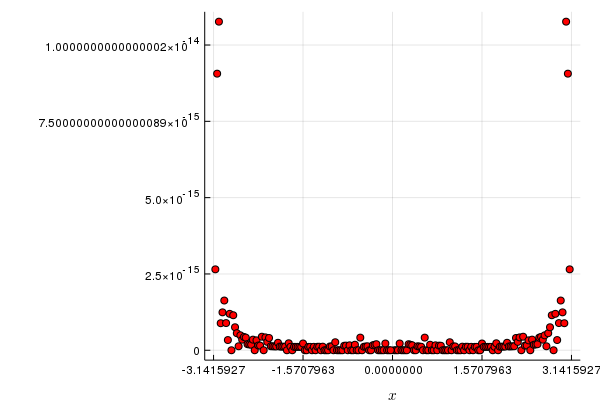
\includegraphics[width=14cm]{sin_Taylor1.png}
  \caption{$\left| \cfrac{sin(x) - sin\_Taylor1(x)}{sin(x)} \right| $}
\end{figure}\\

Jak widać na wykresie wyniki uzyskane dla argumentów bliskich $-\pi$ oraz $\pi$ znacznie bardziej różnią się od oczekiwanych niż te w środku tego przedziału. Przyczyną tego jest fakt, że dla skrajnych argumentów funkcja $sin(x)$ zbiega do $0$, a więc błąd względny rośnie do nieskończoności (w szczególności wartość błędu względnego w punktach $-\pi$, $0$ i $\pi$ nie została w takim razie przedstawiona na wykresie). Dlatego też dla lepszej czytelności i przejrzystości wykresów będę skupiał się na arumentach oddalonych od miejsc zerowych o więcej niż $\cfrac{\pi}{1000}$. Po usunięciu tych skrajnych wartości Rysunek 1 prezentuje się następująco:\\
\\

\begin{figure}[h!]
  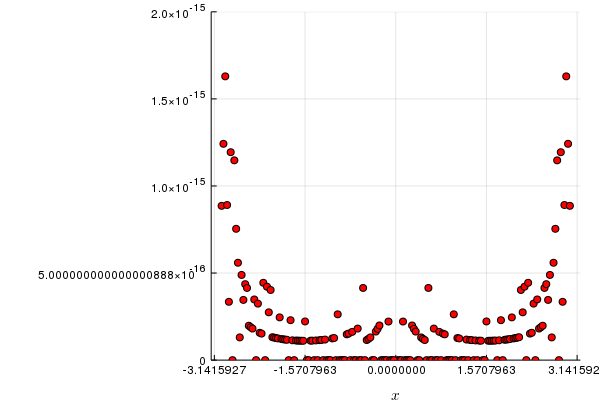
\includegraphics[width=14cm]{sin_Taylor1cut.png}
  \caption{$\left| \cfrac{sin(x) - sin\_Taylor1(x)}{sin(x)} \right| $}
\end{figure}
\pagebreak

Błąd względny rośnie, gdy wartość $sin(x)$ zbliża się do $0$. Dla większości punktów jest on jednak równy $0$ lub mniejszy od $ 5 \cdot 10^{16}$.\\\\

\begin{figure}[h!]
  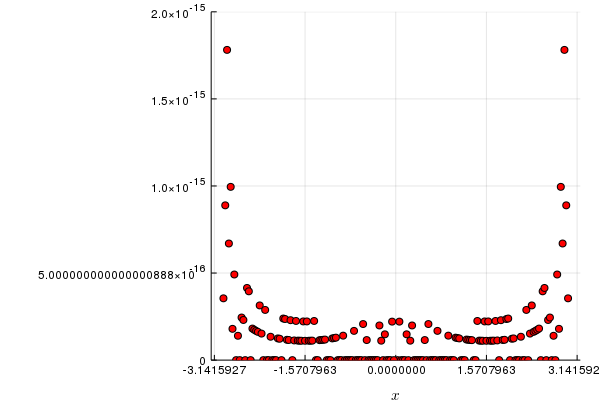
\includegraphics[width=14cm]{sin_Taylor2.png}
  \caption{$\left| \cfrac{sin(x) - sin\_Taylor2(x)}{sin(x)} \right| $}
\end{figure}

Jak widać wykres ten jest bardzo podobny do Rysunku 2. Widać nieznaczną poprawę, zwłaszcza ponownie w okolicach punktów $-\pi$, $0$ i $\pi$. Zaledwie dla dwóch wartości funkcji błąd jest rzędu większego niż $10^{-15}$. Niestety, dla pozostałych wartości różnice między uzyskanymi wartościami są niemalże niezauważalne. Można się było tego spodziewać, gdyż metoda jest \textit{de facto} ta sama, wzór został tylko nieznacznie przekształcony.\\\

\begin{figure}[h!]
  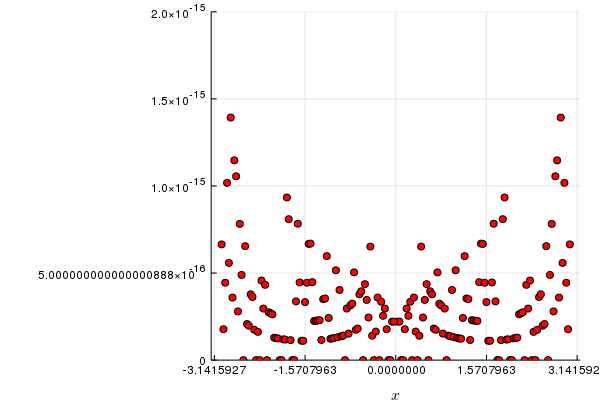
\includegraphics[width=13cm]{sin_fraction.png}
  \caption{$\left| \cfrac{sin(x) - sin\_fraction(x)}{sin(x)} \right| $}
\end{figure}

Wyniki funkcji $sin\_fraction(x)$ są zauważalnie gorsze od wyników uzyskanych ze wzoru Taylora. Procent punktów, których błąd jest zerowy jest znacznie mniejszy, wzrosła za to liczba tych w przedziale $ \left[ \cfrac{1}{2} \cdot 10^{-16}, 10^{-16} \right] $. Jest to zaskakujący wniosek, zważając na fakt, że celem było tak przedstawić ułamek łańcuchowy, by wykonywać możliwie mało dzieleń, co miało zapewnić dużą precyzję wyniku.\\\\

\begin{figure}[h!]
  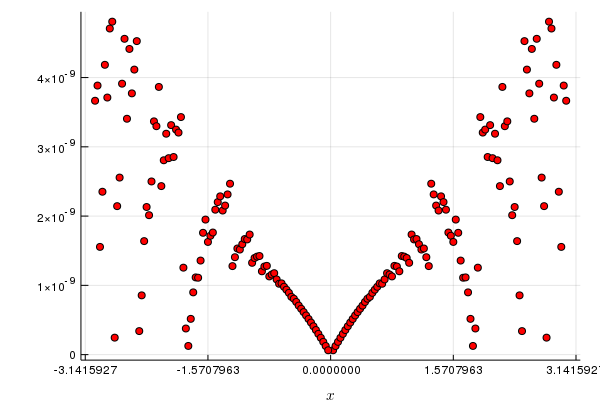
\includegraphics[width=11cm]{sin_mult.png}
  \caption{$\left| \cfrac{sin(x) - sin\_mult(x)}{sin(x)} \right| $}
\end{figure}
\newpage

Ostatnia metoda okazała się najgorszą. Błąd względny dla funkcji $sin\_mult(x)$ wynosi nawet do $4 \cdot 10^9$, co jest o około $7$ rzędów wielkości gorsze od pozostałych metod. Może to wynikać z wielokrotnie wykonywanego dzielenia i odejmowania, które zwłaszcza przy niewielkich liczbach może mieć znaczący wpływ na wynik. Problemem może być też fakt, że dla pozostałych wzorów błędy z każdego wyrazu się dodają, podczas gdy we wzorze \eqref{sinmult} błędy z poszczególnych czynników należy ze sobą przemnożyć,co dodatkowo zwiększa błąd względny.\\

\large
\textbf{4.2. Funkcja $cos(x)$}\\\\
\normalsize
Mało zaskakującym faktem jest, że uzyskane wyniki dla funkcji $cos(x)$ były bardzo podobne do tych uzyskanych dla funkcji $sin(x)$. Również tu największe niedokładności wystąpiły w pobliżu zer funkcji, w tym wypadku $-\cfrac{\pi}{2}$ oraz $\cfrac{\pi}{2}$. 

Na poniższym wykresie porównałem błędy względne wyników uzyskanych dla funkcji $cos\_Taylor1(x)$(kolor czerwony) oraz $cos\_Taylor2(x)$ (kolor niebieski):\\\\

\begin{figure}[h!]
  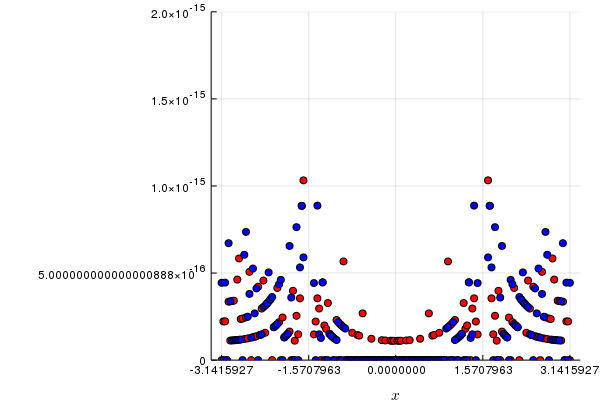
\includegraphics[width=10cm]{cosinus.png}
\end{figure}

Podobnie jak dla sinusa wyniki są bardzo podobne, przy czym dla wersji przenawiasowanej są nieznacznie lepsze. 
\begin{figure}[h!]
  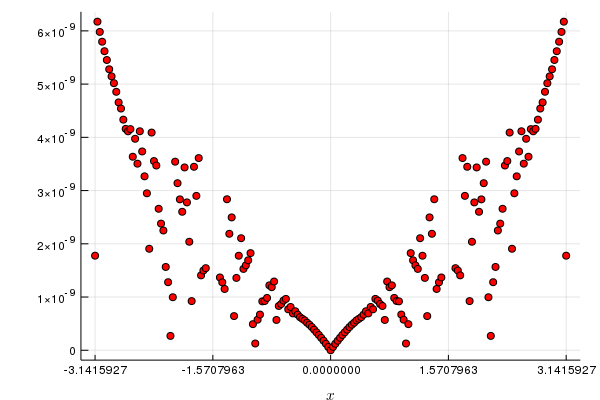
\includegraphics[width=10cm]{cos_mult.png}
  \caption{$\left| \cfrac{cos(x) - cos\_mult(x)}{cos(x)} \right| $}
\end{figure}

Błąd względny funkcji $cos\_mult(x)$ rośnie wraz ze wzrostem wartości bezwzględnej argumentu. Jest on jednak siedem rzędów wielkości większy, niż ten otrzymany za pomocą wzoru Taylora.\\
\Large
\textbf{5. Wnioski}\\
\normalsize

Z przeprowadzonych eksperymentów wynika, że zastosowania wzoru Taylora daje najlepsze efekty przy przybliżaniu funkcji $sin(x)$ i $cos(x)$. Da się te wyniki nieznacznie polepszać poprzez lekkie modyfikacje tego wzoru, ale uzyskiwane wyniki są porównywalne i są bliskie precyzji arytmetyki $u = 1,11 \cdot 10^{-16}$. Nieco gorsze rezultaty daje zastosowanie ułamka łańcuchowego. Jest to zaskakujący wniosek, ponieważ z uwagi na strukturę tego wzoru (niewielka liczba odejmowań i dzieleń) przed wykonaniem doświadczenia mogło się wydawać, że to on będzie najdokładniejszy. Najgorsze rezulataty, zgodnie z przewidywaniami, dało przybliżanie iloczynem, w którym duża liczba odejmowań i dzieleń, zwłaszcza dla liczb, dla których wynik tych operacji jest bliski zeru, znacznie zaburzyła wynik. Stosowanie tej metody może skutkować znacznymi błędami numerycznymi.\\

Okazuje się więc, że jesteśmy w stanie z dokładnością bliską dokładności arytmetyki przybliżać funkcje $sin(x)$ i $cos(x)$ w dowolnym punkcie (jako że są one cykliczne co $2\pi$ i przez to wystarczy, że umiemy je obliczać na przedziale $ \left[ -\pi, \pi \right] $) bez użycia funkcji bibliotecznych.


\newpage
\begin{thebibliography}{9}
\itemsep2pt
\bibitem{MP} M. Paluszyński $"$Analiza Matematyczna dla informatyków. Notatki z wykładu$"$

\bibitem{CO} C. Olds $"$Continued Fractions$"$, wyd. 1963, str. 138

\bibitem{WI} Za Wikipedią: \url{https://pl.wikipedia.org/wiki/Funkcje_trygonometryczne#Definicja_za_pomoc%C4%85_iloczyn%C3%B3w_niesko%C5%84czonych}

\end{thebibliography}

\end{document}